\subsection{Requisito 2}
    \label{subsec:result_req2}
Com base nos resultados do Requisito~\ref{subsec:result_req1} e considerando que: (a) não há uma base para comparação e (b) as imagens não estão necessariamente retificadas; o algoritmo~\emph{Janela Deslizante} com blocos de tamanho $15$ foi selecionado para este requisito. Dessa forma, a exploração aconteceu sobre o tamanho da janela de busca $M \in [100, 800]$, por também ser desconhecida para esta base.

Com isso, os mapas de disparidade não apresentaram bons resultados visuais, uma vez que não é possível vislumbrar uma similaridade com as imagens originais, como demonstrado na Figura~\ref{fig:result_req2_disp_map}. Com o intuito de melhorar o desempenho, as imagens correspondes tiveram o mesmo pré-processamento das imagens do primeiro requisito, sendo realizada uma busca pelos ponto-chaves e suas correspondências entre as imagens, com a finalidade de identificar as linhas epipolares, seguida pela retificação das imagens considerando as suas próprias homografias.

\begin{figure}[!ht]
    \centering
    \begin{tabular}{ccc}
        \bmvaHangBox{\fbox{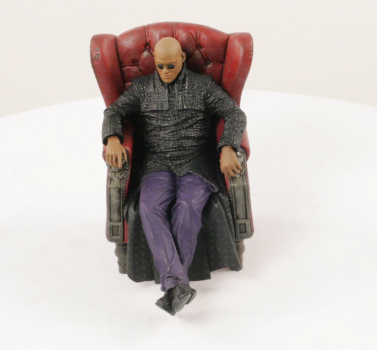
\includegraphics[width=3.5cm]{Figs/Resultados/MorpheusL_rsz.jpg}}}&
        \bmvaHangBox{\fbox{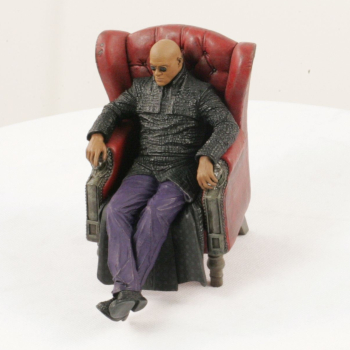
\includegraphics[width=3.5cm]{Figs/Resultados/MorpheusR_rsz.jpg}}}&
        \bmvaHangBox{\fbox{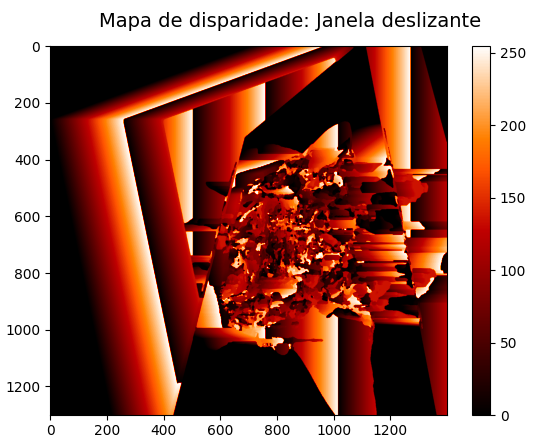
\includegraphics[width=3.5cm]{Figs/Resultados/morpheus_lk400.png}}}\\
        (a)&(b)&(c) \\
        \bmvaHangBox{\fbox{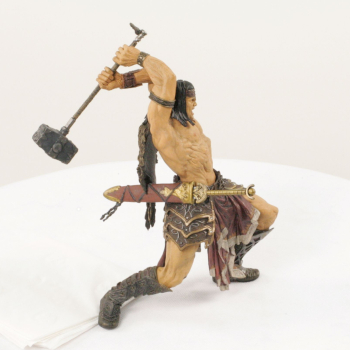
\includegraphics[width=3.5cm]{Figs/Resultados/warriorL_rsz.jpg}}}&
        \bmvaHangBox{\fbox{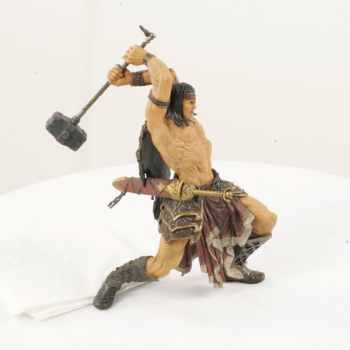
\includegraphics[width=3.5cm]{Figs/Resultados/warriorR_rsz.jpg}}}&
        \bmvaHangBox{\fbox{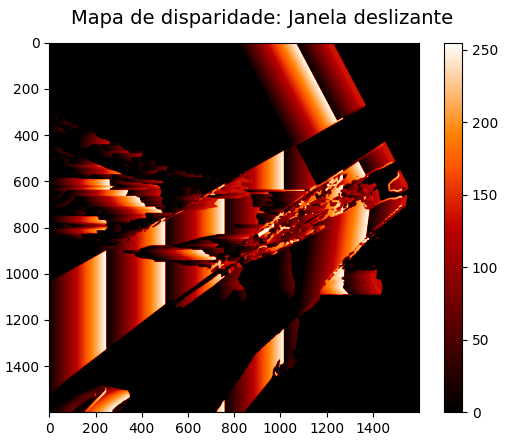
\includegraphics[width=3.5cm]{Figs/Resultados/warrior_lk400.png}}}\\
        (d)&(e)&(f)
    \end{tabular}
    \caption{Mapas de disparidade para o Requisito~\ref{subsec:result_req2}, onde (a) e (d) são as imagens base, (b) e (e) são as imagens correspondentes e (c) e (f) os mapas de disparidade com uma busca de até $400$~\emph{pixels} calculados para o ``Morpheus'' e ``Warrior'', respectivamente. Fonte das imagens (a), (b), (d) e (e) para a base de imagens desativada supracitada.}
    \label{fig:result_req2_disp_map}
\end{figure}

